\documentclass[journal,12pt,twocolumn]{IEEEtran}
\usepackage{graphicx}
\graphicspath{{./figs/}}{}
\usepackage{amsmath,amssymb,amsfonts,amsthm}
\usepackage{multicol}
\usepackage{romannum}
\usepackage{physics}
\usepackage{booktabs}
\usepackage{hyperref}
\newcommand{\myvec}[1]{\ensuremath{\begin{pmatrix}#1\end{pmatrix}}}

\let\vec\mathbf

\title{
Matrix-Lines
}
\author{Akana Sai Kumar}
\begin{document}
\maketitle
\tableofcontents
\bigskip
\section{Problem Statement}
Let A(2,-3) and B(-2, 3) be vertices ofa triangle ABC. If
the centroid of this triangle moves on the line
2x+3y =1, then the locus of the vertex C is the line.\\
\section{Construction}
\begin{figure}[h]
    \centering
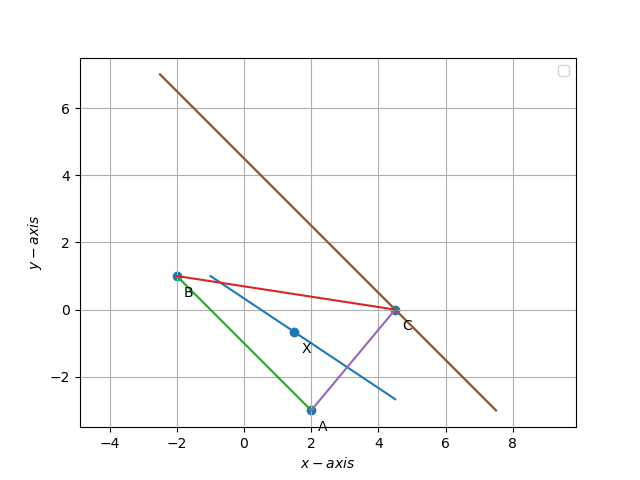
\includegraphics[width=\columnwidth]{mat1.png}
    \caption{Triangle}
    \label{fig:my_label}
\end{figure}
\vspace{2cm}
\begin{table}[h]
    \centering
    \begin{tabular}{|c|c|c|}
       \hline
       \textbf{Symbol}&\textbf{Value}&\textbf{Description}  \\
       \hline
	    $\vec{A}$ & $\myvec{2\\-3}$
	    & Vertex A\\
        \hline
	    $\vec{B}$ & $\myvec{-2\\1}$
 & Vertex B\\
        \hline
	    $\vec{C}$ & $\myvec{h\\k}$
 & Vertex C\\
        \hline
    \end{tabular}
    \caption{Parameters}
    \label{tab:my_label}
\end{table}


\section{Solution}
Given the centroid of this triangle moves on the line 2x+3y =1 \\
\\
\begin{equation}
\vec{X} = \frac{\vec{A}+\vec{B}+\vec{C}}{3}
\end{equation}
\\
Equation of line is 
${\vec{n^{\top}}\vec{X}} = c$.\\
\begin{equation}
	\vec{n^{\top}}(\frac{\vec{A}+\vec{B}+\vec{C}}{3}) = 1 \label{eq-1}
\end{equation}
\\
\begin{equation}
	\vec{n^{\top}}(\vec{A}+\vec{B}+\vec{C}) = 3  \label{eq-2}
\end{equation}
\\
\begin{equation}
	\vec{n^{\top}}\vec{C} = 3 - \vec{n^{\top}}(\vec{A}+\vec{B})
 \label{eq-3}
\end{equation}
\begin{center}
$\vec{n}$ = \myvec{2\\3} \\
 $\vec{A}$ and $\vec{B}$ are given
\end{center}
\begin{equation}
c_1 = 3 - \vec{n^{\top}}(\vec{A}+\vec{B})
\end{equation}
	\begin{equation}
	\vec{n^{\top}}\vec{C}= c_1 \label{eq-4}
\end{equation}
 \\
 The locus of the vertex C is the line\\

 

\section{Software}
\begin{table}[h]
    \centering
    \begin{tabular}{|c|}
    \hline 
    https://github.com/19pa1a0405/sai1729/blob/main/matrices/p.py  \\
        \hline
    \end{tabular}
\end{table}
\section{Conclusion}
We found the equation of a line passing trough a Vertex of $\vec{C}$
is
\begin{equation}
\vec{n^{\top}}\vec{C} = c_1
\end{equation}
\end{document}
